\documentclass[11pt]{article}
\usepackage{amsmath, amssymb, graphicx, booktabs, array}
\usepackage{geometry}
\usepackage{tikz}
\usetikzlibrary{positioning, arrows.meta}
\geometry{margin=1in}
\title{Learning Macroeconomic Policy via Reinforcement Learning: \\ A Dynamic Control Approach (Demo) }
\author{}
\date{}

\begin{document}

\maketitle

\begin{abstract}
We propose a reinforcement learning (RL) framework in which a neural policy learns to conduct macroeconomic stabilization policy in a simulated dynamic economy. The economy is modeled as a stochastic, nonlinear system with lagged responses, expectations formation, and fiscal-monetary interactions. Using a Soft Actor-Critic (SAC) architecture, the agent learns continuous policy interventions that optimize a multi-objective welfare function balancing inflation, unemployment, growth, and debt sustainability. We benchmark against rule-based policies and evaluate robustness under structural shocks.
\end{abstract}

\section{Introduction}
Macroeconomic policy is fundamentally a dynamic control problem under uncertainty. Classical approaches (e.g., Taylor rules, DSGE optimization) rely on fixed functional forms and strong assumptions. In contrast, reinforcement learning offers a data-driven method for discovering adaptive policies in nonlinear environments. This paper formalizes macroeconomic stabilization as a Markov Decision Process and investigates whether an RL agent can learn robust policy rules.

\section{MDP Formulation}
We define the system as:
\begin{align}
    s_{t+1} = f(s_t, a_t, \epsilon_t), \quad r_t = R(s_t, a_t)
\end{align}
where $\epsilon_t$ is a stochastic shock.
This is the basic reinforcement learning picture. At each time step, the agent observes the current state $s_t$, takes an action $a_t$, and the environment responds by moving to a new state $s_{t+1}$ and giving a reward $r_t$. Unlike ordinary supervised learning, there is no correct label telling the model the perfect action in each situation. Instead, the agent has to discover a good policy by trial and error. The goal is not to maximize reward just for one step, but to choose actions that lead to high reward over a long sequence of future steps. That is why RL is naturally suited to policy problems where today's move affects tomorrow's situation.

\subsection{State Space}
\begin{align}
    s_t = [\pi_t, u_t, g_t, r_t, d_t, \mathbb{E}_t\pi_{t+1}, \tau_t, G_t]
\end{align}
The state is the information the agent gets to see before it acts. In ML language, you can think of this as the feature vector fed into the network. A useful state should summarize everything important about the current situation so that the agent can make a sensible decision. In this project, the state contains inflation, unemployment, growth, the interest rate, debt, expected inflation, the tax rate, and the level of government spending. Together these variables give the agent a snapshot of both current macro conditions and the policy stance already in place.

\subsection{Action Space}
\begin{align}
    a_t = [\Delta r_t, \Delta G_t, \Delta \tau_t]
\end{align}
The action is what the agent controls. Here the action is continuous, not discrete, which means the model is not choosing from a short menu like ``raise'' or ``cut.'' Instead it outputs real-valued changes to the policy instruments. That makes the problem closer to regression than classification, but the training signal is still reward-based rather than label-based. Continuous action spaces are one reason we use SAC later: it is a popular RL algorithm designed specifically to learn smooth policies in continuous control tasks.

\section{Economic Model}

\subsection{Aggregate Demand with Lag}
\begin{align}
    g_t = \alpha_1 G_{t-1} - \alpha_2 r_{t-1} + \epsilon_t^d
\end{align}
This equation says that current GDP growth is driven by last period's policy stance plus a random demand disturbance. Government spending enters with a positive sign because extra public spending directly adds to demand for goods and services, which tends to raise output. The interest rate enters with a negative sign because higher borrowing costs discourage household consumption and business investment. The lag matters because policy does not work instantly: a rate rise today does not cancel investment plans immediately, and new government spending projects also take time to filter through the economy. The shock term $\epsilon_t^d$ captures unexpected swings in private demand, such as a collapse in consumer confidence or a sudden borrowing boom.

\subsection{Expectations-Augmented Phillips Curve}
\begin{align}
    \pi_t = \mathbb{E}_t\pi_{t+1} + \beta (g_t - g^*) + \epsilon_t^s
\end{align}
This is the model's inflation equation. It says inflation depends partly on what people expect inflation to be, and partly on whether the economy is running hotter or colder than its normal sustainable speed $g^*$. If growth is above $g^*$, firms face stronger demand, tighter labor markets, and more pricing power, so inflation tends to rise. If growth is below $g^*$, those pressures weaken and inflation tends to fall. The expectations term matters because wage bargaining and price-setting are forward-looking: if firms and workers think inflation will be high, they behave in ways that help make it high. The supply shock $\epsilon_t^s$ captures cost-side surprises such as an energy spike, a shipping disruption, or a sudden fall in productivity.

\subsection{Expectations Formation (Adaptive)}
\begin{align}
    \mathbb{E}_t\pi_{t+1} = \rho \pi_t + (1-\rho) \mathbb{E}_{t-1}\pi_t
\end{align}
This equation explains where inflation expectations come from. Rather than assuming households and firms know the true model, we assume they learn gradually from what they have recently seen. The parameter $\rho$ controls how quickly expectations react to current inflation. A high $\rho$ means people update their beliefs aggressively, so a recent inflation surge quickly changes what they expect next. A low $\rho$ means beliefs are sticky and slow to move. This mechanism is important because it creates persistence: once inflation rises, expectations may also rise, and then those expectations feed back into the Phillips curve above.

\subsection{Okun's Law}
\begin{align}
    u_t = u_{t-1} - \gamma (g_t - g^*)
\end{align}
This is the unemployment equation. It says that what really matters for labor market improvement is not just positive growth, but growth relative to the economy's normal pace $g^*$. If the economy grows faster than its trend, firms usually need more workers, so unemployment falls. If growth is weak relative to trend, firms hire less or even lay workers off, so unemployment rises. The parameter $\gamma$ measures how sensitive unemployment is to growth surprises. This creates the core stabilization trade-off in the model: policy that boosts demand can lower unemployment, but through the Phillips curve it may also push inflation up.

\subsection{Debt Dynamics}
\begin{align}
    d_t = d_{t-1} + G_t - \tau_t
\end{align}
This equation tracks the government debt ratio in a very stripped-down way. Debt today equals debt yesterday plus spending minus tax revenue. If the government spends more than it collects, it runs a deficit and debt rises; if it collects more than it spends, debt falls. In a richer university-level model, debt dynamics would usually include interest payments, the size of GDP, and sometimes separate cyclical tax bases. Here we keep it simple so the strategic trade-off is easy to see: fiscal support can stabilize output in the short run, but persistent deficits eventually worsen debt sustainability.

\subsection{Policy Accumulation}
\begin{align}
    r_t &= r_{t-1} + \Delta r_t \\
    G_t &= G_{t-1} + \Delta G_t \\
    \tau_t &= \tau_{t-1} + \Delta \tau_t
\end{align}
These equations explain what the agent actually controls. It does not choose the full level of rates, spending, or taxes from scratch every quarter; instead it chooses how much to change them. That is more realistic because real policymakers typically make incremental adjustments rather than resetting the whole economy in one move. It also creates inertia in policy: a sequence of small positive $\Delta r_t$ moves can gradually build up into a tight monetary stance, while repeated negative fiscal changes can slowly produce austerity. This accumulation rule is one reason the environment becomes dynamic and path-dependent: today's decision changes tomorrow's starting point.

\section{Reward Function}
In the milestone-one simulator, welfare is scored relative to policy targets:
\begin{align}
    r_t = - w_1 (\pi_t - \pi^*)^2 - w_2 (u_t - u^*)^2 + w_3 (g_t - g^*) - w_4 (d_t - d^*)
\end{align}
The reward is the agent's learning signal. In supervised learning, the loss tells the model how wrong its prediction was relative to a known answer. In RL, there usually is no known best action, so we instead design a reward that expresses what ``good performance'' means. Here, the agent is rewarded when inflation, unemployment, growth, and debt are close to desirable targets. The squared terms mean being far from target is punished more heavily than being slightly off target. Once the reward is defined, the RL algorithm tries to learn a policy that maximizes expected cumulative reward over time, not just the immediate reward from one quarter.

\section{SAC Objective}
\begin{align}
    J(\pi) = \mathbb{E}\left[\sum_t r_t + \alpha H(\pi(\cdot|s_t))\right]
\end{align}
Here $\pi$ means the policy: the rule that maps states to actions. So $J(\pi)$ means ``how good is this whole policy?'' More precisely, it is the expected long-run performance of the policy when we let it interact with the economy over time. The expectation symbol $\mathbb{E}$ appears because outcomes are random: the policy may sample different actions, and the economy itself contains shocks. So SAC is not optimizing one single path of the economy; it is optimizing average performance across many possible trajectories.

The first term inside $J(\pi)$ is the sum of rewards over time, so if a policy keeps inflation and unemployment near target while supporting growth and containing debt, its $J(\pi)$ will be high. The second term uses entropy, written as $H(\pi(\cdot|s_t))$. Entropy measures how spread out or random the policy is. SAC adds this term so the policy keeps exploring instead of collapsing too early onto one narrow behavior. The coefficient $\alpha$ controls how much we care about exploration relative to pure reward.

The Q-function is not written explicitly inside this formula, but it is how SAC makes this objective trainable. In principle, to improve $\pi$, we would like to know which actions lead to high future reward. That long-run usefulness is exactly what the critic estimates through
\[
Q(s_t,a_t) \approx \mathbb{E}\left[\sum_{k=t}^{T} \gamma^{\,k-t} r_k \,\middle|\, s_t, a_t\right].
\]
So you can think of $J(\pi)$ as the overall target we want to maximize, and $Q(s,a)$ as the critic's learned tool for judging which local action choices help increase that target. The actor improves $\pi$ by shifting probability toward actions that the critic scores highly, while SAC still keeps some randomness through the entropy term.

\section{Neural Network Architecture}

\subsection{Actor (Policy)}
\begin{itemize}
    \item Input: $s_t$
    \item Architecture: MLP with 2--3 hidden layers
    \item Output: Gaussian policy parameters $(\mu, \sigma)$
\end{itemize}
The actor is the network that actually chooses actions. Since you already know MLPs, you can think of the actor as an MLP that maps the state vector to a distribution over actions. In SAC, the actor usually outputs the mean $\mu$ and scale $\sigma$ of a Gaussian distribution, then an action is sampled from that distribution. This is useful because the agent needs exploration: early in training it should try different actions rather than committing too quickly to one fixed rule. Later, as learning improves, the sampled actions become concentrated around better decisions.

\subsection{Critic (Q-function)}
\begin{itemize}
    \item Input: $(s_t, a_t)$
    \item Output: $Q(s_t, a_t)$
\end{itemize}
The critic is a separate network that evaluates actions rather than choosing them. Its job is to estimate the \emph{Q-function}, which means the expected total future reward obtained by taking action $a_t$ in state $s_t$ and then continuing with the current policy. The discount factor $\gamma \in (0,1)$ makes near-future rewards count a bit more than distant-future rewards, which keeps the sum well behaved and reflects the idea that immediate consequences are usually more certain than very distant ones. This is the key RL idea that differs from ordinary regression: the model must learn not only whether an action helps right now, but whether it leads to better downstream states. The actor proposes actions, and the critic scores how promising those actions are in long-run terms.

\subsection{SAC Architecture Diagram}
\begin{figure}[ht]
\centering
\small
\begin{tabular}{
    >{\raggedright\arraybackslash}p{0.22\linewidth}
    >{\raggedright\arraybackslash}p{0.33\linewidth}
    >{\raggedright\arraybackslash}p{0.35\linewidth}
}
\toprule
\textbf{SAC relation} & \textbf{Information used} & \textbf{Role in this project} \\
\midrule
Environment interaction
&
The policy observes $s_t=[\pi_t,u_t,g_t,r_t,d_t,\mathbb{E}_t\pi_{t+1},\tau_t,G_t]$ and samples $a_t=(\Delta r_t,\Delta G_t,\Delta \tau_t)$.
&
The macro environment applies the policy move and returns $(r_t,s_{t+1})$. This creates the raw experience used for learning. \\
\midrule
Replay buffer
&
Transitions $(s_t,a_t,r_t,s_{t+1})$ collected from previous economy rollouts.
&
SAC samples mini-batches from this memory so the critic and actor learn from many past macroeconomic situations, not only the latest quarter. \\
\midrule
Critic update
&
The critic estimates $Q_\theta(s_t,a_t)$ and compares it with an entropy-adjusted target value built from $r_t$ and $s_{t+1}$.
&
This trains the Q-function to judge whether a policy action improves long-run macroeconomic welfare. Practical SAC usually uses two critics to reduce overestimation. \\
\midrule
Actor update
&
The actor samples a candidate action $a'_t\sim\pi_\phi(\cdot|s_t)$ and receives the critic score $Q_\theta(s_t,a'_t)$ plus the entropy term.
&
This shifts the policy toward actions with higher estimated long-run value while preserving exploration through the entropy bonus. \\
\bottomrule
\end{tabular}
\caption{SAC architecture represented as a relation map. This table replaces a dense arrow diagram so that the same dependencies are visible without overlapping labels or crossed feedback arrows.}
\end{figure}

This figure should now be read as the SAC training flow for your macroeconomic policy environment. The policy sees the macro state $s_t=[\pi_t,u_t,g_t,r_t,d_t,\mathbb{E}_t\pi_{t+1},\tau_t,G_t]$ and outputs the three policy moves $(\Delta r_t,\Delta G_t,\Delta \tau_t)$. The environment returns a reward and next state, and the transition is stored in the replay buffer. The critic loop learns $Q_\theta(s_t,a_t)$ by comparing it with a target value built from $r_t$, $s_{t+1}$, the target network, and the entropy-adjusted next action. The actor loop samples actions from the current policy, asks the critic how good they are, and then updates the policy toward higher-value actions while still preserving exploration through the entropy term. For readability the figure shows one critic, but the learning logic is consistent with the SAC setup used in this project.

\section{Training Algorithm}
\noindent\textbf{Soft Actor-Critic for Policy Learning}
\begin{enumerate}
    \item Initialize networks and replay buffer.
    \item For each episode:
    \begin{enumerate}
        \item Reset the environment.
        \item For $t = 1$ to $T$:
        \begin{enumerate}
            \item Sample action $a_t \sim \pi(s_t)$.
            \item Observe $s_{t+1}$ and $r_t$.
            \item Store the transition.
            \item Update the critic via Bellman loss.
            \item Update the actor via policy gradient.
        \end{enumerate}
    \end{enumerate}
\end{enumerate}
The training loop ties the whole RL system together. Each pass through the environment generates experience tuples of the form $(s_t, a_t, r_t, s_{t+1})$. These are stored in a replay buffer, which is just a memory bank of past transitions. Instead of learning only from the most recent step, SAC samples batches from this buffer and uses gradient descent to update the networks. The critic is trained to better predict long-run value, usually through a Bellman-style target that bootstraps from estimated future values. The actor is then updated to place more probability on actions that the critic says have high value. So the big picture is: collect experience, improve the critic's judgment, then improve the actor using that judgment.

\section{Experimental Design}

\subsection{Baselines}
\begin{itemize}
    \item Taylor rule
    \item Random policy
\end{itemize}

\subsection{Shock Scenarios}
\begin{itemize}
    \item Demand shocks ($\epsilon^d$)
    \item Supply shocks ($\epsilon^s$)
    \item Structural breaks
\end{itemize}

\subsection{Metrics}
\begin{itemize}
    \item Variance of inflation
    \item Variance of unemployment
    \item Mean GDP growth
    \item Debt trajectory
    \item Cumulative welfare
\end{itemize}

\section{Ablation Studies}
We analyze:
\begin{itemize}
    \item Effect of removing expectations
    \item Effect of removing lag structure
    \item Sensitivity to reward weights
\end{itemize}

\section{System Diagram}
\begin{center}
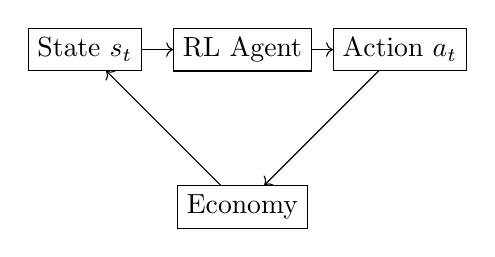
\begin{tikzpicture}[node distance=2cm]
\node (state) [draw] {State $s_t$};
\node (agent) [draw, right of=state] {RL Agent};
\node (action) [draw, right of=agent] {Action $a_t$};
\node (env) [draw, below of=agent] {Economy};
\draw[->] (state) -- (agent);
\draw[->] (agent) -- (action);
\draw[->] (action) -- (env);
\draw[->] (env) -- (state);
\end{tikzpicture}
\end{center}

\section{Discussion}
This framework highlights the role of learning-based control in macroeconomics. Challenges include model misspecification, reward alignment, and generalization under structural change.

\section{From Macroeconomic Control to a General Failure Question}
The macroeconomic simulator provides one concrete instance of a broader class of controlled Markov systems. In the more general setting considered here, the state is a vector $s_t \in \mathbb{R}^n$, the action is produced by a policy $\pi$, and the system evolves according to
\begin{align}
    s_{t+1} = f(s_t, \pi(s_t)).
\end{align}
The target of control is a prescribed state $s^*$, and performance is measured by a distance-based loss such as
\begin{align}
    L(s_t,s^*) = \|s_t - s^*\|_2^2.
\end{align}
The central research question is not only whether RL can reduce this loss in practice, but under what structural conditions \emph{any} policy can make the trajectory converge to the target. This reformulation matters because policy failure can arise from the system itself, rather than from poor training alone.

\subsection{Why Equilibrium Feasibility Must Be Checked First}
Before studying learning, one must determine whether the target can even be maintained once reached. If no action can hold the system at $s^*$, then the learning problem is ill-posed: the loss cannot converge to zero because the target is not a feasible steady state of the dynamics.

Let $u^*$ denote the action applied at the target. A necessary condition for feasibility is
\begin{align}
    s^* = f(s^*,u^*), \qquad u^* \in \mathcal{U},
\end{align}
where $\mathcal{U}$ is the admissible action set. This formula is needed because it separates two distinct difficulties. The first is optimization: whether an algorithm can discover a good policy. The second is feasibility: whether the target is compatible with the physical, economic, or institutional constraints of the system. If no admissible $u^*$ satisfies this fixed-point equation, then failure is structural. In that case, even an ideal optimizer cannot make $L(s_t,s^*) \to 0$.

\subsection{Why a Lyapunov View Is Needed}
Reward trajectories alone do not establish stability. Reinforcement learning can produce temporarily good reward while the state remains fragile, oscillatory, or only conditionally stable. A Lyapunov function is introduced because it provides a direct mathematical test of whether deviations from the target shrink over time.

Once a policy is fixed, the controlled system becomes the closed-loop map
\begin{align}
    s_{t+1} = g(s_t) := f(s_t,\pi(s_t)).
\end{align}
The natural candidate Lyapunov function for this project is the same distance-based quantity used in the loss:
\begin{align}
    V(s_t) = L(s_t,s^*) = \|s_t - s^*\|_2^2.
\end{align}
This choice is important because it links the machine learning objective and the stability objective. The function $V$ is positive definite around $s^*$: it is zero at the target and positive elsewhere. The next step is to study its one-step difference,
\begin{align}
    \Delta V(s_t) = V(s_{t+1}) - V(s_t)
    = \|g(s_t)-s^*\|_2^2 - \|s_t-s^*\|_2^2.
\end{align}
This formula is needed because the sign of $\Delta V$ expresses the local direction of the error energy. If $\Delta V(s_t) < 0$ for all $s_t$ in a neighborhood of $s^*$ except at the target itself, then the closed-loop system is locally asymptotically stable in that neighborhood. If $\Delta V$ becomes positive in some directions, then the distance to the target grows rather than shrinks, and the policy cannot stabilize the system there.

\subsection{Why Local Linearization Is Introduced}
For a high-dimensional nonlinear system, the exact expression for $\Delta V$ is often too complicated to analyze directly. Local linearization is introduced because it replaces the nonlinear dynamics by a first-order approximation near the target, making the source of failure mathematically visible.

Define the local deviations
\begin{align}
    \Delta s_t = s_t - s^*, \qquad \Delta u_t = u_t - u^*.
\end{align}
Assuming that $f$ is differentiable near $(s^*,u^*)$, a first-order Taylor expansion gives
\begin{align}
    \Delta s_{t+1}
    \approx
    A \Delta s_t + B \Delta u_t,
\end{align}
with
\begin{align}
    A = \left.\frac{\partial f}{\partial s}\right|_{(s^*,u^*)},
    \qquad
    B = \left.\frac{\partial f}{\partial u}\right|_{(s^*,u^*)}.
\end{align}
This pair of matrices has a clear interpretation. The matrix $A$ describes how the system's own internal couplings propagate local deviations even when the action is held fixed. The matrix $B$ describes how strongly the control channel can influence those deviations. In intuitive terms, $A$ measures endogenous instability or persistence, while $B$ measures control authority.

\subsection{Why the Closed-Loop Matrix $G=A+BK$ Appears}
The linearized model above still contains the action increment $\Delta u_t$. To study stabilization, the policy must also be approximated locally. If the policy is differentiable near the target, then
\begin{align}
    \Delta u_t \approx K \Delta s_t,
    \qquad
    K = \left.\frac{\partial \pi}{\partial s}\right|_{s^*}.
\end{align}
This formula is needed because it converts the abstract policy into a local feedback gain matrix. Substituting it into the linearized dynamics yields
\begin{align}
    \Delta s_{t+1} \approx (A+BK)\Delta s_t.
\end{align}
The matrix
\begin{align}
    G = A + BK
\end{align}
is the local closed-loop transition matrix. It is important because it gathers the system dynamics and the policy into one object. Stability is then determined by whether this matrix contracts deviations or amplifies them.

Using the simple quadratic candidate $V(\Delta s_t)=\|\Delta s_t\|_2^2$, the Lyapunov difference becomes
\begin{align}
    \Delta V(\Delta s_t)
    \approx
    \Delta s_t^\top (G^\top G - I)\Delta s_t.
\end{align}
This identity is needed because it makes the local stabilization requirement algebraic. A sufficient condition for decrease of this specific quadratic Lyapunov function is
\begin{align}
    G^\top G - I \prec 0.
\end{align}
More generally, local asymptotic stability of the linearized closed loop is characterized by
\begin{align}
    \rho(G) < 1,
\end{align}
where $\rho(G)$ is the spectral radius of $G$. Equivalently, there exists some positive definite matrix $P$ such that
\begin{align}
    G^\top P G - P \prec 0.
\end{align}
This more general form matters because the Euclidean distance is not always the correct geometry for a coupled system. In applications such as macroeconomics, the state variables may have different scales and economic meanings, so a weighted quadratic form can be more informative than the raw Euclidean norm.

\subsection{Why Controllability Must Be Introduced}
Even if the closed-loop matrix $G$ determines local stability, this still does not answer whether a suitable feedback gain can exist. Controllability is introduced because it formalizes whether the control inputs can influence all relevant state directions of the linearized system.

Starting from
\begin{align}
    \Delta s_{t+1} = A\Delta s_t + B\Delta u_t,
\end{align}
one may expand the dynamics across several steps:
\begin{align}
    \Delta s_1 &= A\Delta s_0 + B\Delta u_0, \\
    \Delta s_2 &= A^2\Delta s_0 + AB\Delta u_0 + B\Delta u_1, \\
    \Delta s_3 &= A^3\Delta s_0 + A^2B\Delta u_0 + AB\Delta u_1 + B\Delta u_2.
\end{align}
Continuing to step $n$ yields
\begin{align}
    \Delta s_n
    =
    A^n\Delta s_0
    + A^{n-1}B\Delta u_0
    + A^{n-2}B\Delta u_1
    + \cdots
    + B\Delta u_{n-1}.
\end{align}
This expansion is needed because it exposes how present and past actions propagate through the coupled state dynamics. Rearranging gives
\begin{align}
    \Delta s_n - A^n\Delta s_0
    =
    \begin{bmatrix}
        B & AB & A^2B & \cdots & A^{n-1}B
    \end{bmatrix}
    \begin{bmatrix}
        \Delta u_{n-1} \\
        \Delta u_{n-2} \\
        \vdots \\
        \Delta u_0
    \end{bmatrix}.
\end{align}
The matrix
\begin{align}
    \mathcal{C}
    =
    \begin{bmatrix}
        B & AB & A^2B & \cdots & A^{n-1}B
    \end{bmatrix}
\end{align}
is the Kalman controllability matrix. It is important because its column space describes all local state directions that can be reached by combining admissible inputs across multiple time steps.

If
\begin{align}
    \mathrm{rank}(\mathcal{C}) < n,
\end{align}
then some state directions are unreachable under the linearized dynamics. In that case, no local feedback policy can fully counteract disturbances in those directions. Even when $\mathrm{rank}(\mathcal{C}) = n$, failure can still occur if the entries of $B$ are extremely small or if the action constraints in $\mathcal{U}$ are tight. Then the system may be controllable in principle but too weakly actuated in practice to overcome shocks, nonlinear drift, or saturation. This directly matches the intuition that a volatile system can fail because policy influence is too small relative to endogenous motion.

\subsection{A Worked Linear Macroeconomic Example}
The previous subsections introduced the general tools. A concrete example is needed because it shows how an apparently reasonable economic model can contain a structural failure mode before any RL algorithm is trained. The simplified macroeconomic system in this paper is already close to linear, so it can be rewritten as an explicit state-space model and analyzed directly.

For this analysis, stochastic shocks are removed and all variables are expressed as deviations from a steady state. This step is not a change in the economic model; it is a coordinate change that makes stability and controllability visible. Let the steady state be
\begin{align}
    (g^*,\pi^*,u^*,d^*,r^*,G^*,\tau^*,e^*),
\end{align}
where $e_t=\mathbb{E}_t\pi_{t+1}$. A feasible steady state must satisfy
\begin{align}
    g^* &= \alpha_1G^*-\alpha_2r^*, \\
    \pi^* &= e^*, \\
    G^* &= \tau^*.
\end{align}
The first condition says that trend growth must be consistent with the steady policy stance. The second says that inflation expectations are correct at the steady state. The third says that debt is constant only when government spending equals tax revenue in this simplified debt equation.

Define deviation variables by placing a tilde over each variable:
\begin{align}
    \tilde g_t &= g_t-g^*, &
    \tilde \pi_t &= \pi_t-\pi^*, &
    \tilde u_t &= u_t-u^*, \\
    \tilde d_t &= d_t-d^*, &
    \tilde r_t &= r_t-r^*, &
    \tilde G_t &= G_t-G^*, \\
    \tilde \tau_t &= \tau_t-\tau^*, &
    \tilde e_t &= e_t-e^*.
\end{align}
In these coordinates, the deterministic economic equations become
\begin{align}
    \tilde g_t &= \alpha_1\tilde G_{t-1}-\alpha_2\tilde r_{t-1}, \\
    \tilde \pi_t &= \tilde e_t+\beta\tilde g_t, \\
    \tilde e_t &= \rho\tilde \pi_t+(1-\rho)\tilde e_{t-1}, \\
    \tilde u_t &= \tilde u_{t-1}-\gamma\tilde g_t, \\
    \tilde d_t &= \tilde d_{t-1}+\tilde G_t-\tilde \tau_t.
\end{align}

The expectation and inflation equations are simultaneous, so it is useful to eliminate $\tilde \pi_t$ before writing the system matrix. Substituting $\tilde e_t=\rho\tilde \pi_t+(1-\rho)\tilde e_{t-1}$ into $\tilde \pi_t=\tilde e_t+\beta\tilde g_t$ gives
\begin{align}
    \tilde \pi_t
    =
    \rho\tilde \pi_t+(1-\rho)\tilde e_{t-1}+\beta\tilde g_t.
\end{align}
Therefore,
\begin{align}
    \tilde \pi_t
    =
    \tilde e_{t-1}
    +
    \frac{\beta}{1-\rho}\tilde g_t.
\end{align}
Let
\begin{align}
    \kappa = \frac{\beta}{1-\rho},
    \qquad
    \eta = \frac{\rho\beta}{1-\rho}.
\end{align}
Then the expectation equation becomes
\begin{align}
    \tilde e_t
    =
    \tilde e_{t-1}+\eta\tilde g_t.
\end{align}
This algebraic reduction matters because it shows that inflation itself is not the only memory channel. Expected inflation is the persistent state variable, and it is moved by the same output-gap channel that also moves unemployment.

Now define the state vector and policy action by
\begin{align}
    x_t
    =
    \begin{bmatrix}
        \tilde u_{t-1} \\
        \tilde e_{t-1} \\
        \tilde d_{t-1} \\
        \tilde r_{t-1} \\
        \tilde G_{t-1} \\
        \tilde \tau_{t-1}
    \end{bmatrix},
    \qquad
    a_t
    =
    \begin{bmatrix}
        \Delta r_t \\
        \Delta G_t \\
        \Delta \tau_t
    \end{bmatrix}.
\end{align}
The output gap and inflation deviation are then read from the state as
\begin{align}
    \tilde g_t
    &=
    \begin{bmatrix}
        0&0&0&-\alpha_2&\alpha_1&0
    \end{bmatrix}x_t, \\
    \tilde \pi_t
    &=
    \begin{bmatrix}
        0&1&0&-\kappa\alpha_2&\kappa\alpha_1&0
    \end{bmatrix}x_t.
\end{align}
The full linear state-space system is
\begin{align}
    x_{t+1} = Ax_t+Ba_t,
\end{align}
where
\begin{align}
    A
    =
    \begin{bmatrix}
        1&0&0&\gamma\alpha_2&-\gamma\alpha_1&0\\
        0&1&0&-\eta\alpha_2&\eta\alpha_1&0\\
        0&0&1&0&1&-1\\
        0&0&0&1&0&0\\
        0&0&0&0&1&0\\
        0&0&0&0&0&1
    \end{bmatrix},
    \qquad
    B
    =
    \begin{bmatrix}
        0&0&0\\
        0&0&0\\
        0&1&-1\\
        1&0&0\\
        0&1&0\\
        0&0&1
    \end{bmatrix}.
\end{align}
This explicit form reveals the economic structure of the model. Interest-rate changes first move the policy-rate state. Spending and tax changes first move the fiscal states. These policy states then affect output, and output affects unemployment and expectations.

\subsection{Kalman Interpretation of the Linear Example}
The Kalman view asks whether policy actions can move every independent state direction. For the six-dimensional system above, the controllability matrix is
\begin{align}
    \mathcal{C}
    =
    \begin{bmatrix}
        B&AB&A^2B&A^3B&A^4B&A^5B
    \end{bmatrix}.
\end{align}
For generic nonzero parameters in the simplified model, this matrix has rank five rather than six:
\begin{align}
    \mathrm{rank}(\mathcal{C}) = 5 < 6.
\end{align}
The rank loss can be understood without computing every column of $\mathcal{C}$. The unemployment and expectation equations imply
\begin{align}
    \tilde u_t &= \tilde u_{t-1}-\gamma\tilde g_t,\\
    \tilde e_t &= \tilde e_{t-1}+\eta\tilde g_t.
\end{align}
Multiplying the first equation by $\eta$ and the second by $\gamma$, then adding them, gives
\begin{align}
    \eta\tilde u_t+\gamma\tilde e_t
    =
    \eta\tilde u_{t-1}+\gamma\tilde e_{t-1}.
\end{align}
Thus
\begin{align}
    q_t = \eta\tilde u_t+\gamma\tilde e_t
\end{align}
is an invariant of the controlled dynamics. No sequence of actions can change this quantity. In vector form, with
\begin{align}
    w =
    \begin{bmatrix}
        \eta\\
        \gamma\\
        0\\
        0\\
        0\\
        0
    \end{bmatrix},
\end{align}
the invariant can be written as $w^\top x_t=q_t$, and the matrices satisfy
\begin{align}
    w^\top A = w^\top,
    \qquad
    w^\top B = 0.
\end{align}
This is exactly the structural obstruction detected by Kalman controllability. Since one linear combination of the state is unchanged by every admissible action sequence, the reachable set from a given initial condition lies on the hyperplane
\begin{align}
    w^\top x = w^\top x_0.
\end{align}
Consequently, the origin can be reached only if $w^\top x_0=0$. If the initial economy has
\begin{align}
    \eta\tilde u_0+\gamma\tilde e_0 \neq 0,
\end{align}
then no policy, learned or hand-designed, can drive all six deviations exactly to zero in this simplified model.

Economically, the failure arises because unemployment and expected inflation are both moved through the same output-gap channel. Policy can influence output through interest rates and spending, but in this simplified structure it cannot independently choose the path of unemployment and the path of expectations. One common lever moves both. This is enough to create an uncontrollable direction even though the model has three policy instruments.

\subsection{Lyapunov Interpretation of the Linear Example}
The Lyapunov view reaches the same conclusion from the stability side. Suppose a local linear policy is applied:
\begin{align}
    a_t = Kx_t.
\end{align}
The closed-loop system is then
\begin{align}
    x_{t+1} = (A+BK)x_t = Gx_t.
\end{align}
For asymptotic stability of the origin in the full six-dimensional state space, the closed-loop matrix must satisfy
\begin{align}
    \rho(G)<1.
\end{align}
Equivalently, there must exist a positive definite matrix $P$ such that
\begin{align}
    G^\top P G - P \prec 0.
\end{align}
However, the invariant found above remains true under every feedback gain $K$. Since $w^\top B=0$,
\begin{align}
    w^\top G
    =
    w^\top(A+BK)
    =
    w^\top A+w^\top BK
    =
    w^\top.
\end{align}
Therefore, $1$ is always a left eigenvalue of the closed-loop matrix $G$. Hence
\begin{align}
    \rho(G)\ge 1
\end{align}
for every possible linear feedback gain. This means that no policy can make the whole six-dimensional deviation vector asymptotically stable at the origin. A Lyapunov function may still decrease on the five-dimensional controllable subspace, but it cannot be strictly decreasing in all nonzero directions of the full state space.

This example connects the two perspectives in a precise chain:
\begin{align}
    \begin{aligned}
    &\text{structural invariant}
    \Longrightarrow
    \mathrm{rank}(\mathcal{C})<6
    \Longrightarrow
    \text{an immovable closed-loop mode} \\
    &\Longrightarrow
    \rho(G)\ge 1
    \Longrightarrow
    \text{no full-state Lyapunov proof of asymptotic stability}.
    \end{aligned}
\end{align}
For the research question of this paper, this is a useful counterexample. It shows that even a linear, low-dimensional, economically interpretable model need not be stabilizable to an arbitrary target from an arbitrary initial condition. If an RL policy fails in such a case, the failure is not necessarily caused by insufficient training or network capacity. It may be caused by the geometry of the controlled Markov process itself.

\subsection{Why Constraint Sets and Viability Are Needed}
In constrained systems, eventual convergence is not the only question. A policy may move the state toward the target in the long run while violating hard limits on the way. Viability theory is introduced because it distinguishes between asymptotic desirability and trajectory-wise admissibility.

Let $\mathcal{X} \subseteq \mathbb{R}^n$ denote the safe set, that is, the set of states consistent with physical, institutional, or social constraints. The viability kernel is
\begin{align}
    \mathrm{Viab}_f(\mathcal{X})
    =
    \left\{
        s_0 \in \mathcal{X}
        \;\middle|\;
        \exists \pi \text{ such that } s_t \in \mathcal{X} \text{ for all } t \ge 0
    \right\}.
\end{align}
This concept is needed because it identifies which initial states are fundamentally recoverable under the given control limits. If $s_0 \notin \mathrm{Viab}_f(\mathcal{X})$, then failure is unavoidable: the trajectory must leave the safe region under every admissible policy before stabilization can occur. In the present project, this corresponds to cases where the initial macroeconomic state is so extreme that no bounded sequence of policy actions can restore the system without violating debt, inflation, or unemployment limits first.

\subsection{Chain of Failure}
The preceding concepts form a single logical chain. Failure of RL-based stabilization does not begin with optimization alone. It can begin much earlier, at the level of feasibility, control authority, or admissible trajectories.

\begin{figure}[ht]
\centering
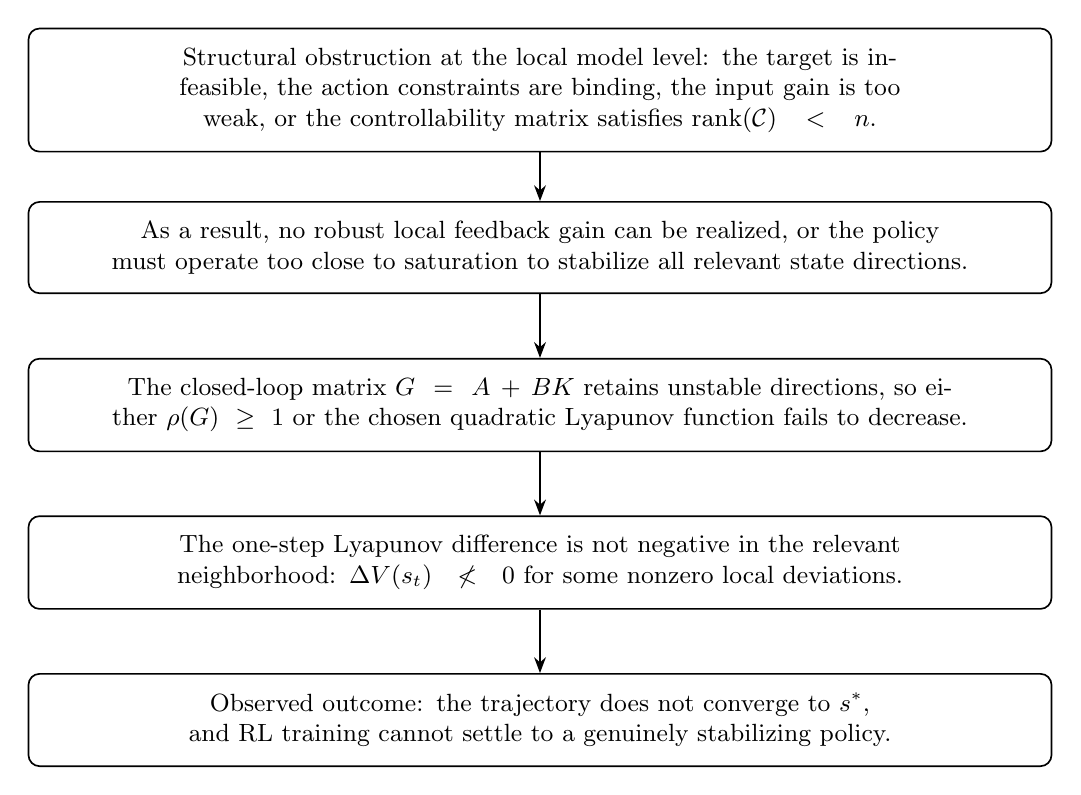
\begin{tikzpicture}[
    >=Stealth,
    semithick,
    font=\small,
    failbox/.style={
        draw,
        rounded corners=4pt,
        align=center,
        text width=12.5cm,
        minimum height=1.1cm,
        inner sep=7pt
    }
]
    \node[failbox] (b1) at (0, 0) {Structural obstruction at the local model level: the target is infeasible, the action constraints are binding, the input gain is too weak, or the controllability matrix satisfies $\mathrm{rank}(\mathcal{C})<n$.};
    \node[failbox] (b2) at (0, -2.0) {As a result, no robust local feedback gain can be realized, or the policy must operate too close to saturation to stabilize all relevant state directions.};
    \node[failbox] (b3) at (0, -4.0) {The closed-loop matrix $G=A+BK$ retains unstable directions, so either $\rho(G)\ge 1$ or the chosen quadratic Lyapunov function fails to decrease.};
    \node[failbox] (b4) at (0, -6.0) {The one-step Lyapunov difference is not negative in the relevant neighborhood: $\Delta V(s_t)\not<0$ for some nonzero local deviations.};
    \node[failbox] (b5) at (0, -8.0) {Observed outcome: the trajectory does not converge to $s^*$, and RL training cannot settle to a genuinely stabilizing policy.};

    \draw[->] (b1) -- (b2);
    \draw[->] (b2) -- (b3);
    \draw[->] (b3) -- (b4);
    \draw[->] (b4) -- (b5);
\end{tikzpicture}
\caption{Logical chain linking structural properties of the controlled system to failure of RL-based stabilization.}
\end{figure}

\subsection{Connection Back to the Present Project}
The macroeconomic environment developed in this project offers a useful testbed because the state variables have real interpretations and the action channels are economically meaningful. In that setting, the reward already resembles a quadratic stabilization objective, so it naturally suggests a Lyapunov-style interpretation. At the same time, the analysis above clarifies an important limitation: successful RL performance in the simulator does not by itself prove that arbitrary coupled Markov systems are stabilizable.

The broader research program is therefore to identify when stabilization fails for structural reasons. Four failure modes are particularly important. First, the target $s^*$ may be infeasible under the admissible action set. Second, the local control authority measured by $B$ may be too weak relative to the intrinsic dynamics measured by $A$. Third, the initial state $s_0$ may lie outside the viability kernel of the constrained system. Fourth, strong nonlinearities may shrink the domain in which the local approximation remains valid, so that a policy that is stabilizing near $s^*$ still fails from more distant initial conditions. These cases define the boundary between a merely trainable controller and a genuinely stabilizing one.

\section{Selected Theoretical Literature}
The present project sits at the intersection of reinforcement learning, nonlinear control, and constrained dynamical systems. Several references are especially relevant to the failure question posed above.

\begin{itemize}
    \item Tsitsiklis and Van Roy, ``Analysis of Temporal-Difference Learning with Function Approximation'' (1996), for early mathematical results showing that value-function learning with function approximation can be unstable.
    \item Dai et al., ``SBEED: Convergent Reinforcement Learning with Nonlinear Function Approximation'' (ICML 2018), for a route toward convergence guarantees under nonlinear approximation.
    \item Zhang et al., ``Provably Convergent Two-Timescale Off-Policy Actor-Critic with Function Approximation'' (ICML 2020), for actor-critic convergence theory closer to modern RL practice.
    \item Boffi et al., ``Learning Stability Certificates from Data'' (CoRL 2021), for learning Lyapunov-style certificates directly from trajectories.
    \item Wan, Naik, and Sutton, ``Learning and Planning in Average-Reward Markov Decision Processes'' (ICML 2021), for a formulation that is often more appropriate than discounted return in continuing control systems.
    \item Moerland et al., ``Model-based Reinforcement Learning: A Survey'' (2022), for a broad overview of approaches that may be better suited to structured dynamical systems than purely model-free methods.
\end{itemize}

\section{Conclusion}
We demonstrate a reinforcement learning approach to macroeconomic policy design. Future work includes multi-agent economies and real-world calibration.

\end{document}
